\section{Verdelingsonderzoek}
\subsection{Univariate steekproeven}
\paragraph{Steekproefgemiddelde} Het steekproefgemiddelde van een steekproef \(X_{1},\dots,X_{n}\) is de stochastische grootheid
\[
    \avg{X}=\frac{1}{n}\sum_{i=1}^{n}X_{i}.
\]

\paragraph{Steekproefvariantie} De steekproefvariantie van een steekproef \(X_{1},\dots,X_{n}\) is de stochastische grootheid
\[
    S_{X}^{2}=\frac{1}{n-1}\sum_{i=1}^{n}\left(X_{i}-\avg{X}\right)^{2}.
\]

\subsection{Histogrammen}
Zij \(X_{1},\dots,X_{n}\) een steekproef met bereik \(R\subseteq\r\) en \(a_{0}<\dots<a_{m}\) een partitie van \(R\). Dan is het histogram van de steekproef op een interval \((a_{j-1},a_{j}]\) gegeven door
\[
    h(x)=\frac{1}{a_{j}-a_{j-1}}\sum_{i=1}^{n}1_{(a_{j-1},a_{j}]}(x_{i}).
\]
Het geschaalde histogram schaalt het histogram met een factor \(\frac{1}{n}\). Het geschaalde histogram is dus gelijk aan
\[
    h(x)=\frac{1}{n(a_{j}-a_{j-1})}\sum_{i=1}^{n}1_{(a_{j-1},a_{j}]}(x_{i}).
\]

\subsection{Boxplots}
\paragraph{Kwartielen} Gegeven een steekproef \(X_{1},\dots,X_{n}\) is net \(n\)-de kwartiel de waarde \(X_{i}\) zodat precies \(\frac{n}{4}\) uitkomsten van de steekproef kleiner zijn dan \(X_{i}\).

\paragraph{Boxplots} Een boxplot is een grafiek waarin de kwartielen van een steekproef weergegeven zijn. Het boxplot van een normaalverdeling ziet er bij benadering uit als in figuur \ref{fig:boxplot_norm}.

\begin{figure}[ht]
    \centering
    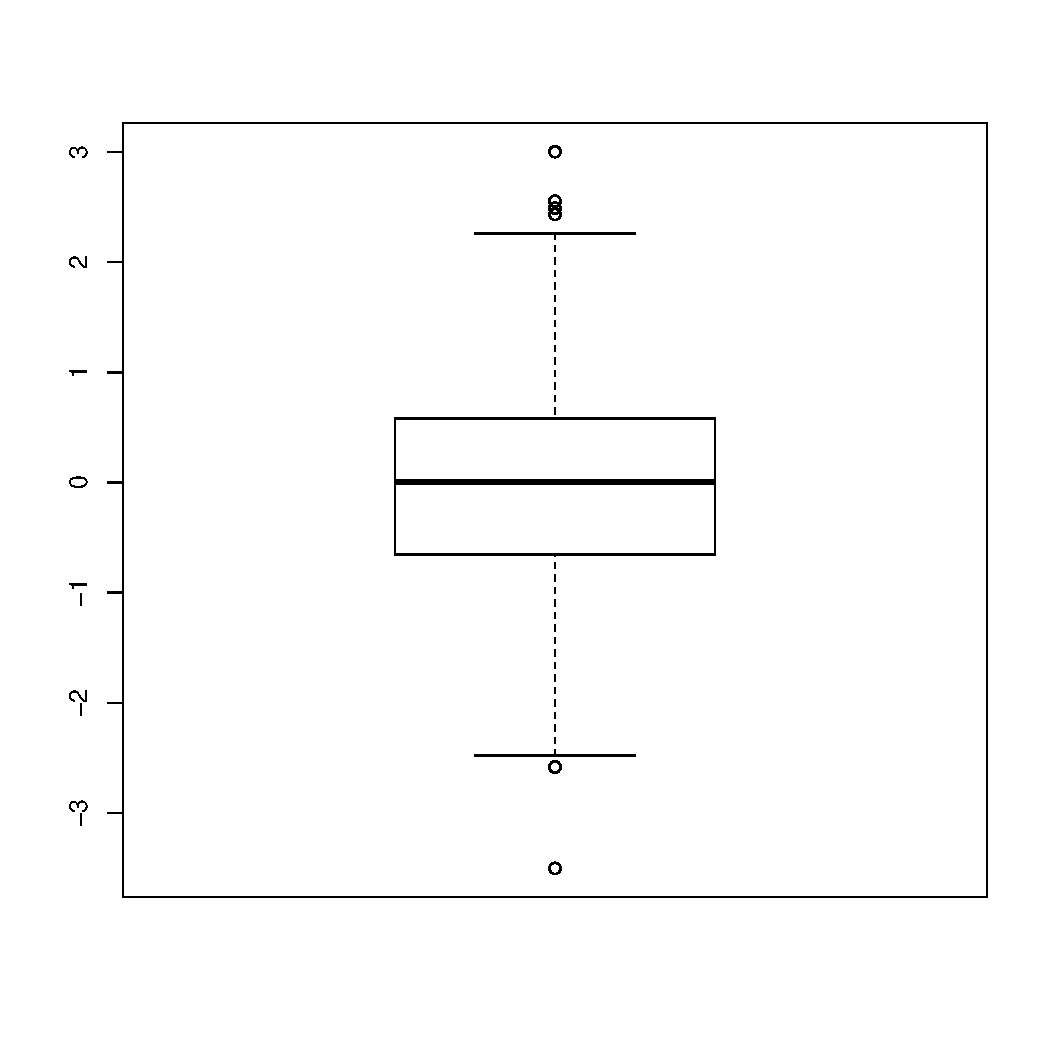
\includegraphics[width=0.7\textwidth]{plots/data.pdf}
    \caption{Een benadering van het boxplot van een normaalverdeling.}
    \label{fig:boxplot_norm}
\end{figure}

\subsection{Locatie schaalfamilie}
\paragraph{Locatie-schaalfamilie} Gegeven een stochastische grootheid \(X\) met verdelingsfunctie \(F\), dan heeft de stochast \(Y=a+bX\) de verdelingsfunctie \(F_{a,b}\) gegeven door
\[
    F_{a,b}(y)=\p(a+bX\leq y)=F\left(\frac{y-a}{b}\right).
\]
De familie kansverdelingen \(\{F_{a,b}\colon a\in\r,b>0\}\) heet de locatie-schaalfamilie behorend bij \(F\) of van \(X\).

\paragraph{Kwantielen} Gegeven een stochast \(X\) met verdelingsfunctie \(F\) is het \(\alpha\)-kwantiel (voor \(\alpha\in(0,1)\)) gelijk aan
\[
    F^{-1}(\alpha)=\inf\{x\colon F(x)\geq\alpha\}.
\]

\paragraph{Ordestatistieken} De ordestatistieken van een steekproef \(X_{1},\dots,X_{n}\) worden gegeven door de rij \(X_{(1)},\dots,X_{(n)}\) zodat ze geplaatst zijn in stijgende volgorde.

Voor de \(i\)-de ordestatistiek geldt dat \(\e F(X_{(i)})=\frac{i}{n+1}\) en algemener geldt dat \(X_{(i)}=a+bF^{-1}\left(\frac{i}{n+1}\right)\) voor \(X_{1},\dots,X_{n}\) elementen verdeeld met \(F_{a,b}\).

\paragraph{QQ-plot} Een QQ-plot van de data \(x_{1},\dots,x_{n}\) ten opzichte van een verdelingsfunctie \(F\) is een grafiek van de punten
\[
    \left\{\left(F^{-1}\left(\frac{i}{n+1}\right),x_{(i)}\right)\mid i=1,\dots,n\right\}.
\]

\subsection{Samenhang}
\paragraph{Scatterplot} Een scatterplot van tweedimensionale data \((x_{1},y_{1}),\dots,(x_{n},y_{n})\) is een grafiek van deze punten in het \(\r^{2}\)-vlak.

\paragraph{Steekproefcorrelatiecoëfficiënt} Het steekproefcorrelatiecoëfficiënt van een steekproef bestaande uit paren \((X_{1},Y_{1}),\dots,(X_{n},Y_{n})\) is
\[
    r_{X,Y}=\frac{\sum_{i=1}^{n}(X_{i}-\avg{X})(Y_{i}-\avg{Y})}{(n-1)\sqrt{S_{X}^{2}}\sqrt{S_{Y}^{2}}}.
\]

Het steekproefcorrelatiecoëfficiënt is een mate van lineairiteit van het verband tussen de waarden \(x_{i}\) en \(y_{i}\).

\paragraph{Auto-correlaties} Gegeven de uitkomst van een steekproef \(x_{1},\dots,x_{n}\) is het auto-correlatiecoëfficiënt een maat van correlatie tussen \(x_{i}\) en \(X_{i-h}\). Het wordt gegeven door
\[
    r_{x}(h)=\frac{\sum_{i=1}^{n-h}(x_{i+h}-\avg{x})(x_{i}-\avg{x})}{(n-h)s_{x}^{2}}.
\]